\section{Overview of the Methodology}
\label{sec:methodologyOverview}

This chapter describes the research design and implementation steps taken to empirically evaluate the impact of selected Explainable Artificial Intelligence (XAI) methods on user trust in Large Language Model (LLM) outputs. As illustrated in Figure~\ref{fig:methodology_overview}, the overall methodology is organized into five sequential stages: the selection of an appropriate LLM, the selection and implementation of XAI methods, the design and execution of a user survey, the evaluation of the collected data, and the development of a prototype implementation. The right-hand column of the figure indicates that each stage is accompanied by documentation of the reasoning behind the choices made. The final stage synthesizes all findings into a results summary. The following sections describe each stage in detail.

\begin{figure}
    \centering
    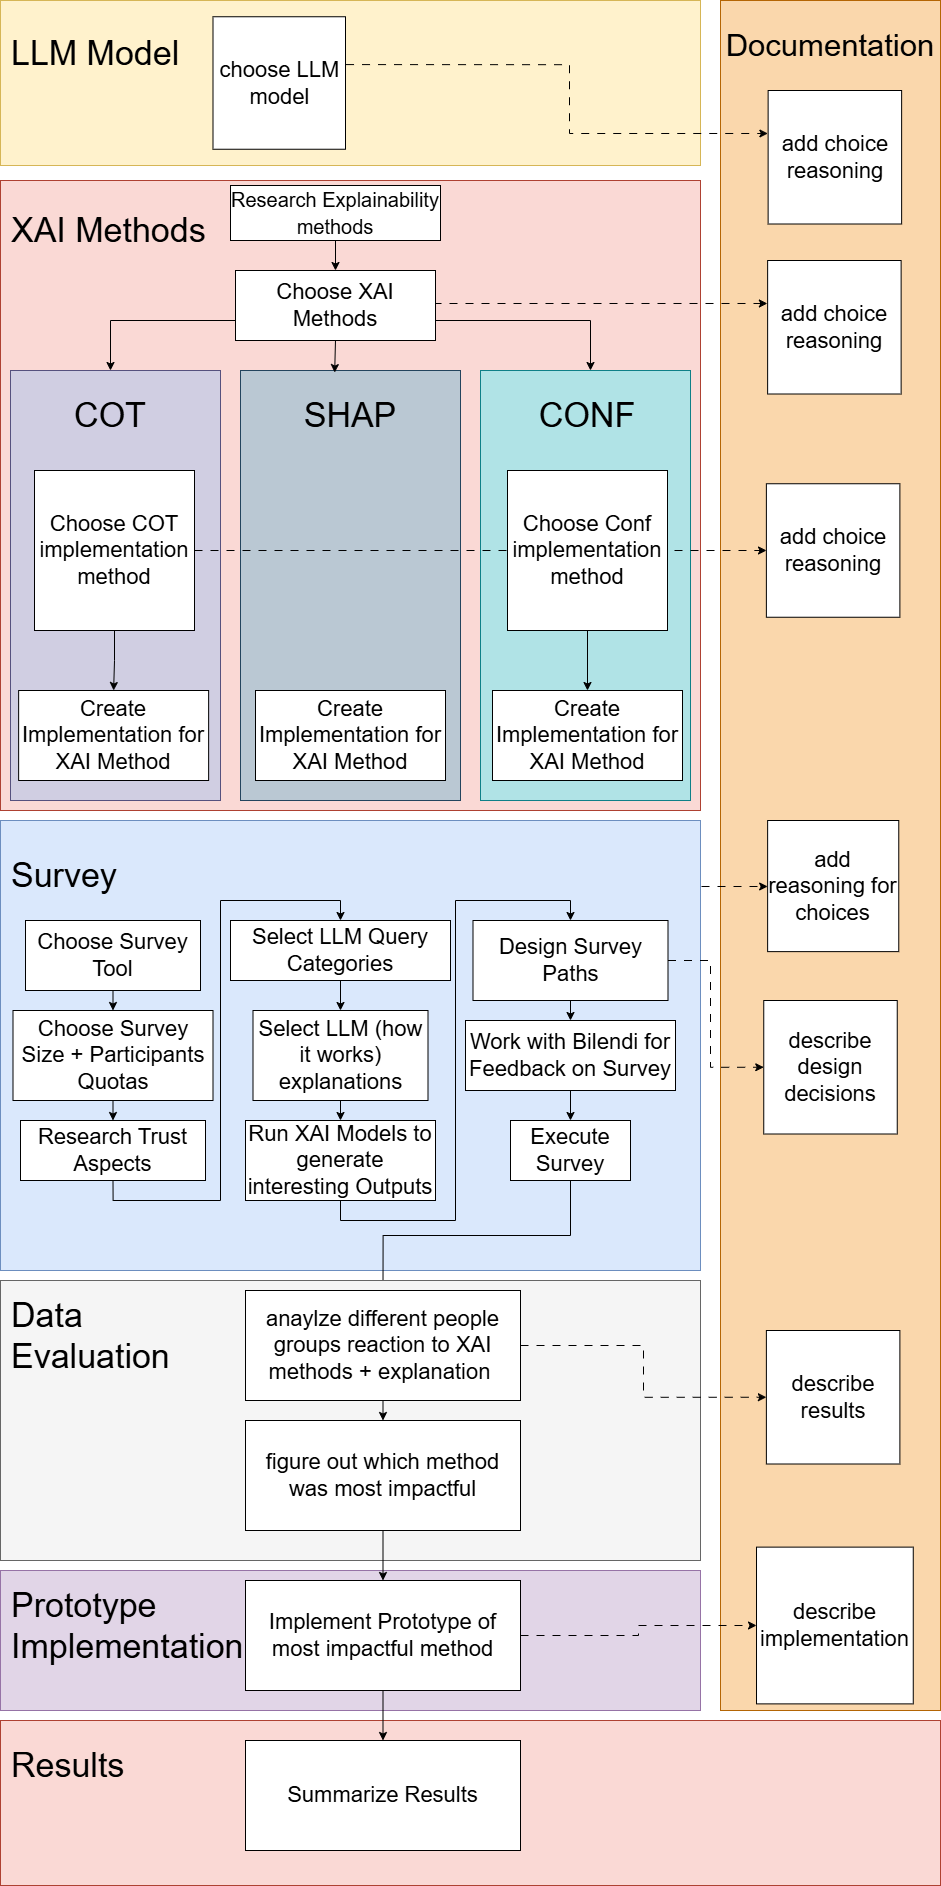
\includegraphics[width=0.7\linewidth]{img/methods.png}
    \caption{Visual Methodology Diagram}
    \label{fig:methodology_overview}
\end{figure}


 TODO 
=> evtl dokumentationspart weglah?

prototyp implementation für umfrage beschreiben => evtl dann: wie es dann für umfrageteilnehmer aussah siehe anhang

\section{Model and Method Selection}
\label{sec:modelandmethod}

\subsection{LLM Selection}

The first step in operationalizing this study was the selection of a suitable LLM to serve as the underlying system whose outputs participants would evaluate. Three criteria guided this decision. First, the model needed to be sufficiently well-known that survey participants might plausibly have encountered it before, which helps ensure that responses to the model's outputs are not confounded by unfamiliarity with the technology itself. Second, the model had to be open-source, or at minimum freely available for research purposes, in order to allow full transparency and reproducibility of the experimental setup. Third, pre-trained weights needed to be publicly accessible, as fine-tuning or training from scratch was outside the scope of this work.

Llama~2 and its successor Llama~3, developed by Meta AI, satisfy all three of these requirements. Both models are released under open licenses that permit research use, their weights and training code are publicly available, and they have achieved sufficient public prominence to be recognized by a broad audience. Furthermore, Llama models support the modification of the system prompt, the instruction passed to the model prior to a user query that shapes its behavior and response style, which is necessary for implementing certain XAI approaches in this study. The models also exist in versions trained with Reinforcement Learning from Human Feedback (RLHF), which improves instruction-following and output quality. For these reasons, Llama 3.1\cite{noauthor_llama_nodate} was selected as the model for this study.

\subsection{XAI Method Selection}

The selection of XAI methods was guided by the goal of covering a representative range of explanation categories as they apply to LLMs, while at the same time ensuring that each method is implementable within the constraints of the study and comprehensible to lay participants without a technical background. Given the particular characteristics of LLMs, which operate on natural language rather than structured tabular data, not all classical XAI approaches are straightforwardly applicable, and the selection had to account for this.

Figure~\ref{fig:xai_categories} illustrates the taxonomy of XAI methods relevant to this context. Based on this categorization, three methods were selected: SHAP-based feature attribution combined with counterfactual reasoning, Chain-of-Thought (CoT) prompting, and confidence indication. As shown in Figure~\ref{fig:methodology_overview}, each of the three methods was implemented independently. Together, these methods span distinct explanation paradigms, covering post-hoc attribution, process transparency, and uncertainty quantification respectively, while remaining accessible to a non-expert audience.

\paragraph{SHAP and Counterfactual Reasoning} 
SHAP (SHapley Additive exPlanations)\cite{lundberg_unified_2017} is a post-hoc attribution method grounded in cooperative game theory that assigns each input token a score reflecting its contribution to the model output. In the context of this study, SHAP scores are presented visually to indicate which parts of a prompt most strongly influenced the model's response. This is complemented by counterfactual reasoning, which illustrates how a change in the input would have altered the output, thereby offering an intuitive causal framing. Figures~\ref{fig:shap_sample} and~\ref{fig:counter_sample} show a representative example as it appeared in the survey.

\FloatBarrier

\begin{figure}
    \centering
    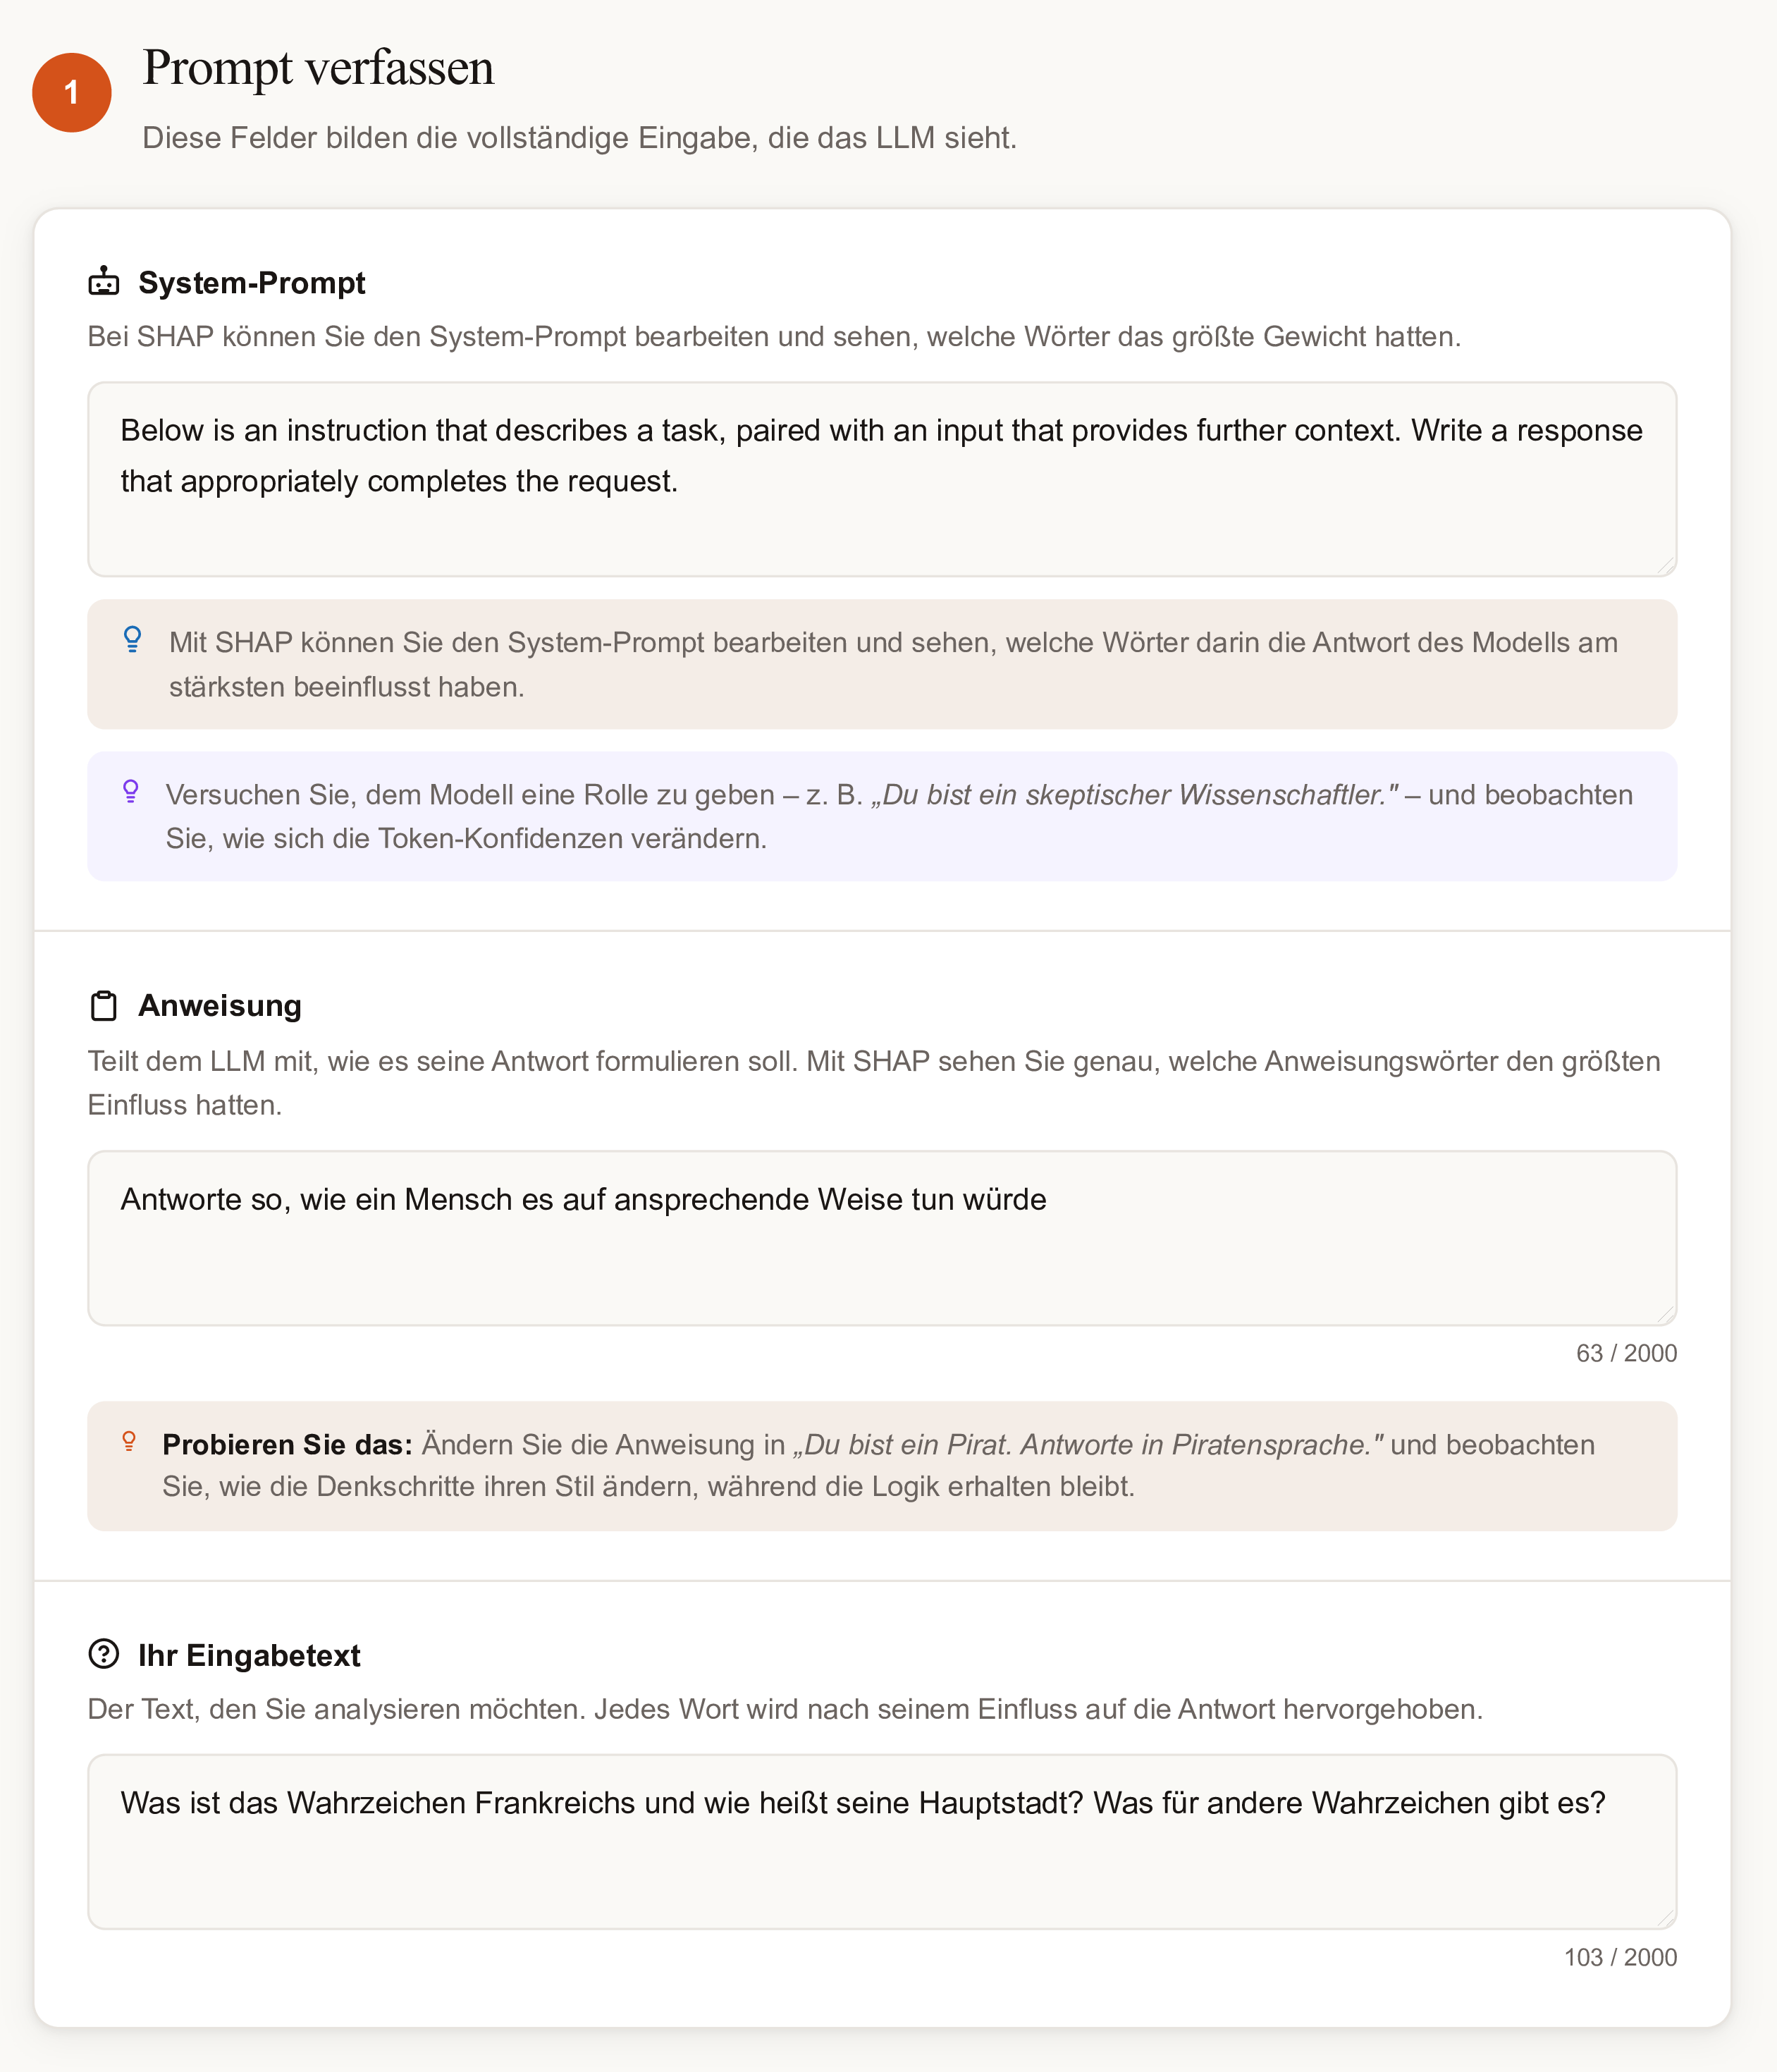
\includegraphics[width=0.7\linewidth]{img/shap_example_p1.png}
    \caption{Query and System Prompt Sample}
    \label{fig:shap_sample}
\end{figure}
\begin{figure}
    \centering
    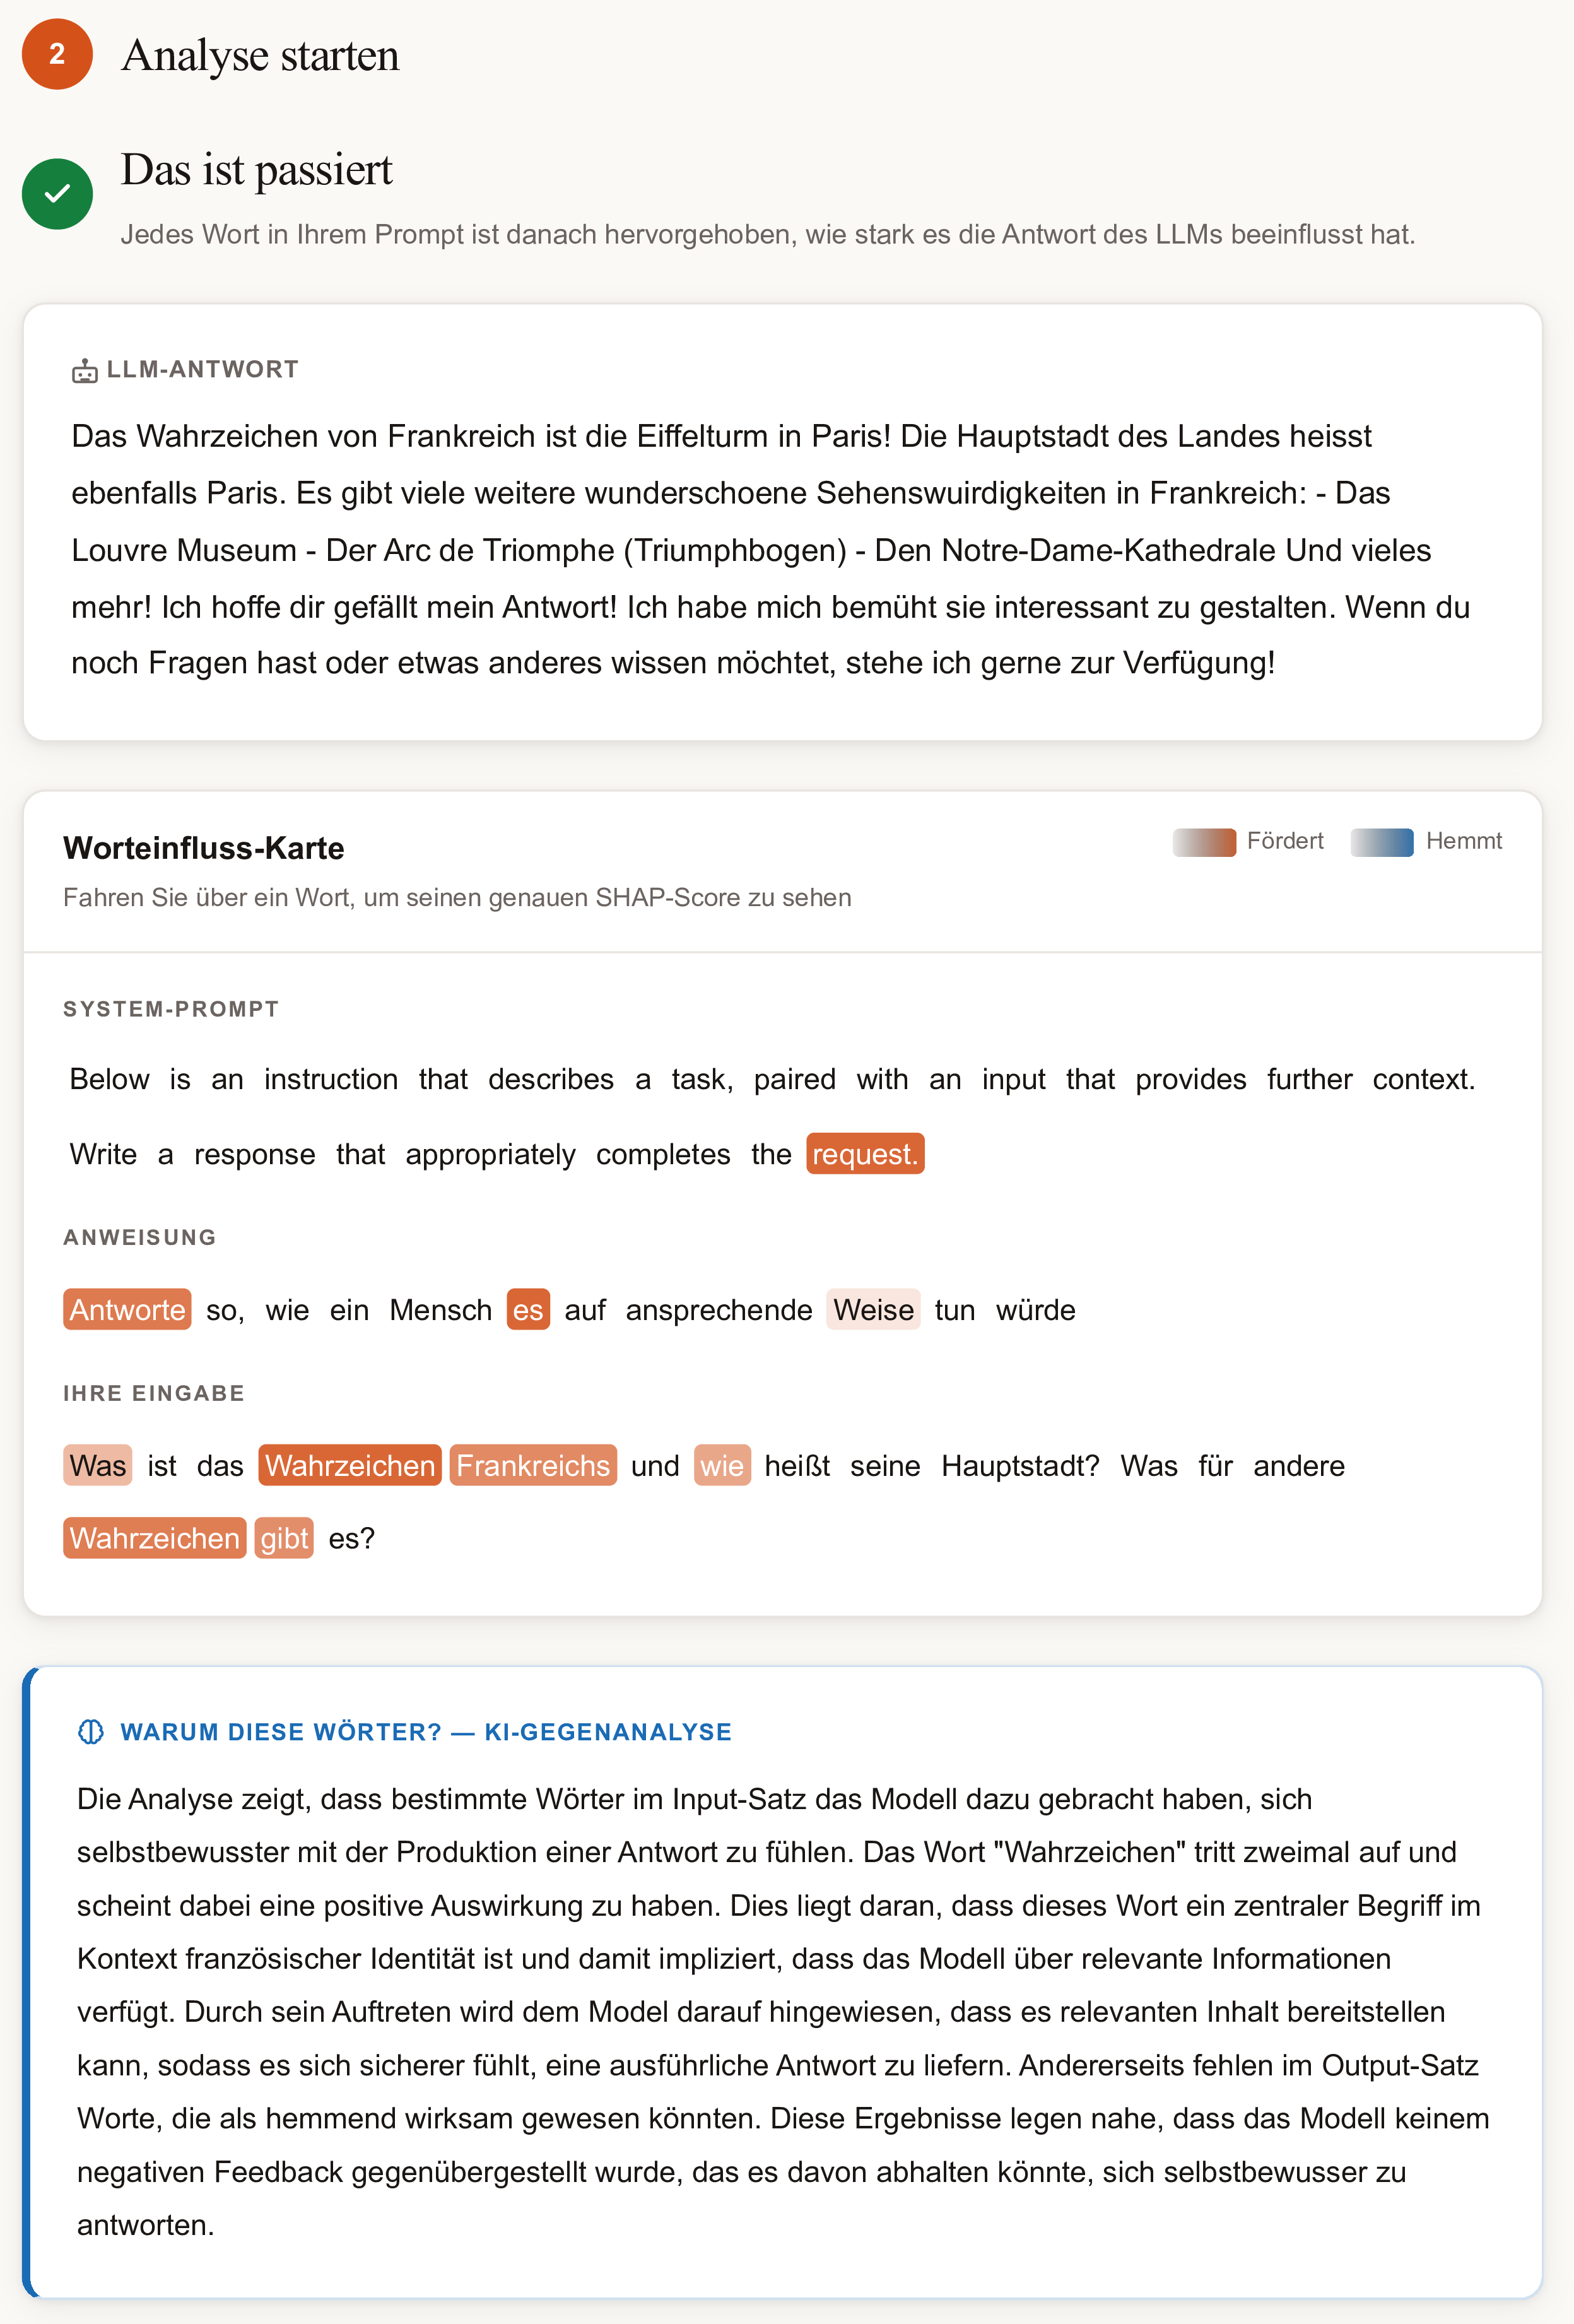
\includegraphics[width=0.7\linewidth]{img/shap_example_p2.png}
    \caption{SHAP and Counterfactual Reasoning Sample}
    \label{fig:counter_sample}
\end{figure}

\FloatBarrier

\paragraph{Chain-of-Thought (CoT)} 
Chain-of-Thought prompting elicits intermediate reasoning steps from the model by instructing it to explain its thinking before arriving at a final answer. Unlike post-hoc explanations, CoT is an intrinsic method in which the explanation is generated as part of the model's output itself. This makes it particularly easy to present to users in a natural, readable format. A sample CoT output as presented in the survey is shown in Figure~\ref{fig:cot_sample}.

\begin{figure}
    \centering
    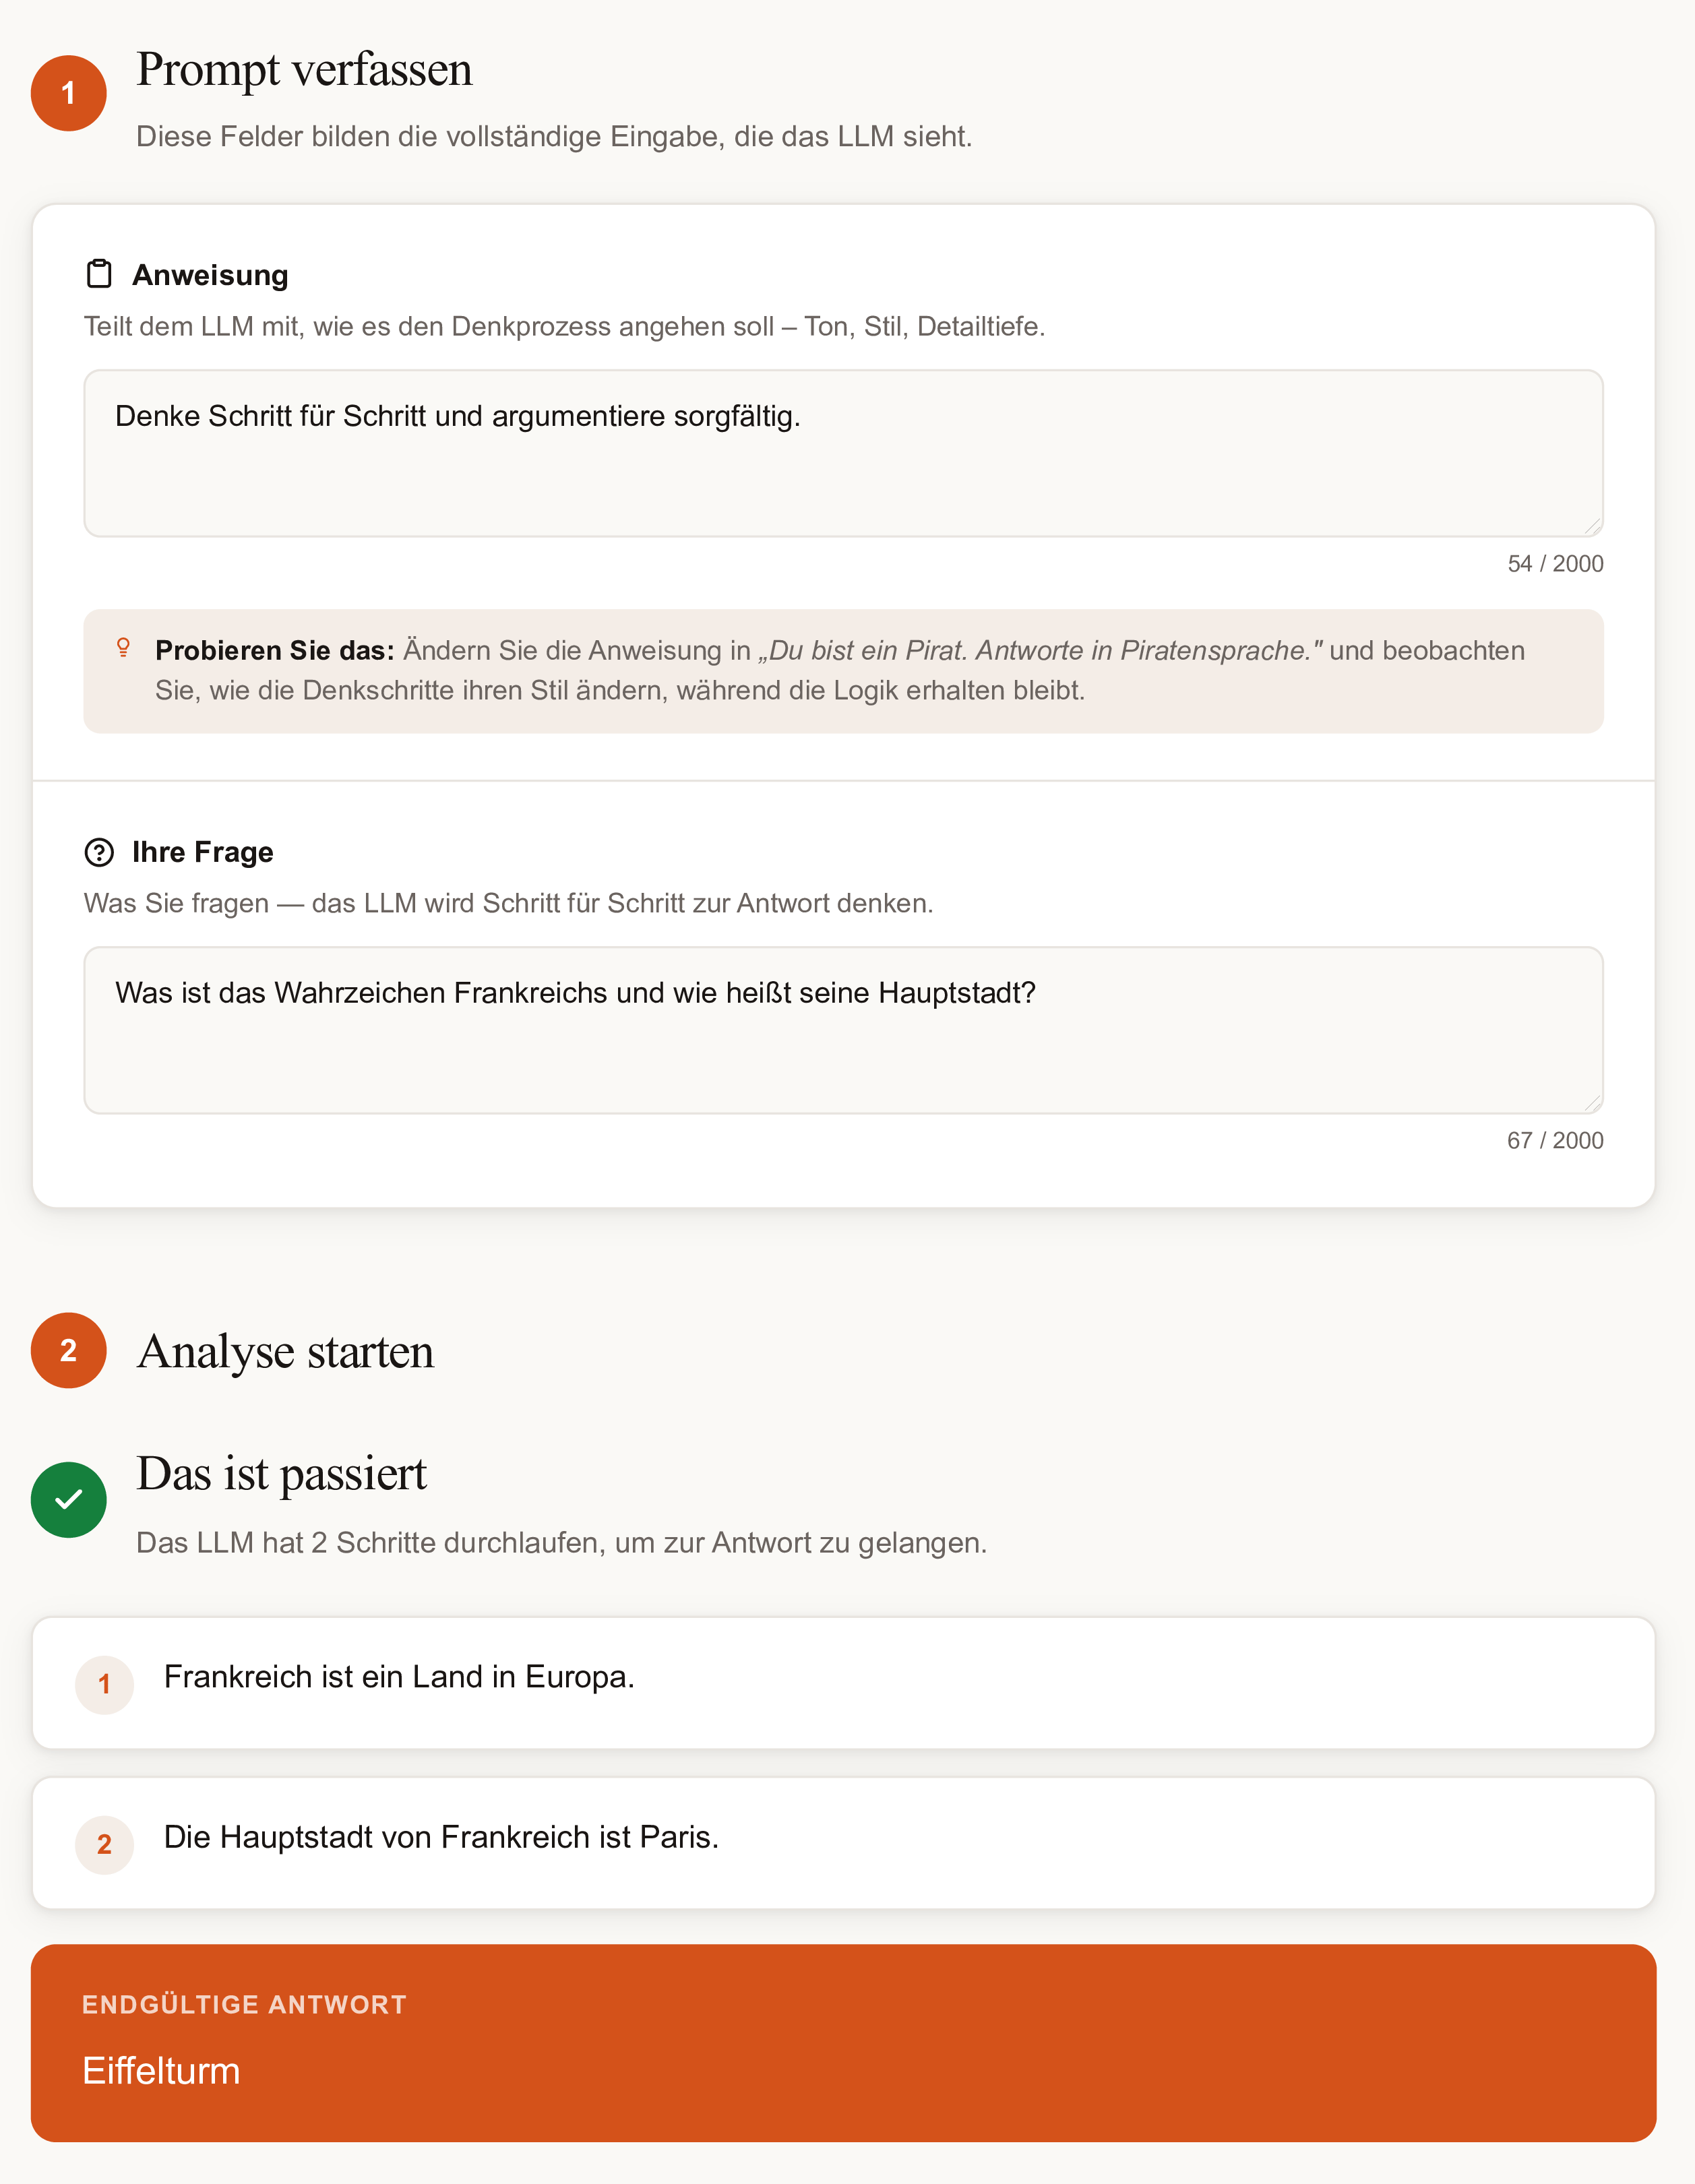
\includegraphics[width=0.7\linewidth]{img/cot_example.png}
    \caption{Chain of Thought Sample}
    \label{fig:cot_sample}
\end{figure}

\paragraph{Confidence Indication} 
Confidence scores provide an estimate of the model's certainty in its output, either derived from token-level probability distributions or expressed through natural language hedging. This method represents a form of uncertainty quantification and communicates the model's epistemic state to the user in a direct and concise way. A sample confidence output is shown in Figure~\ref{fig:conf_sample}.

\begin{figure}
    \centering
    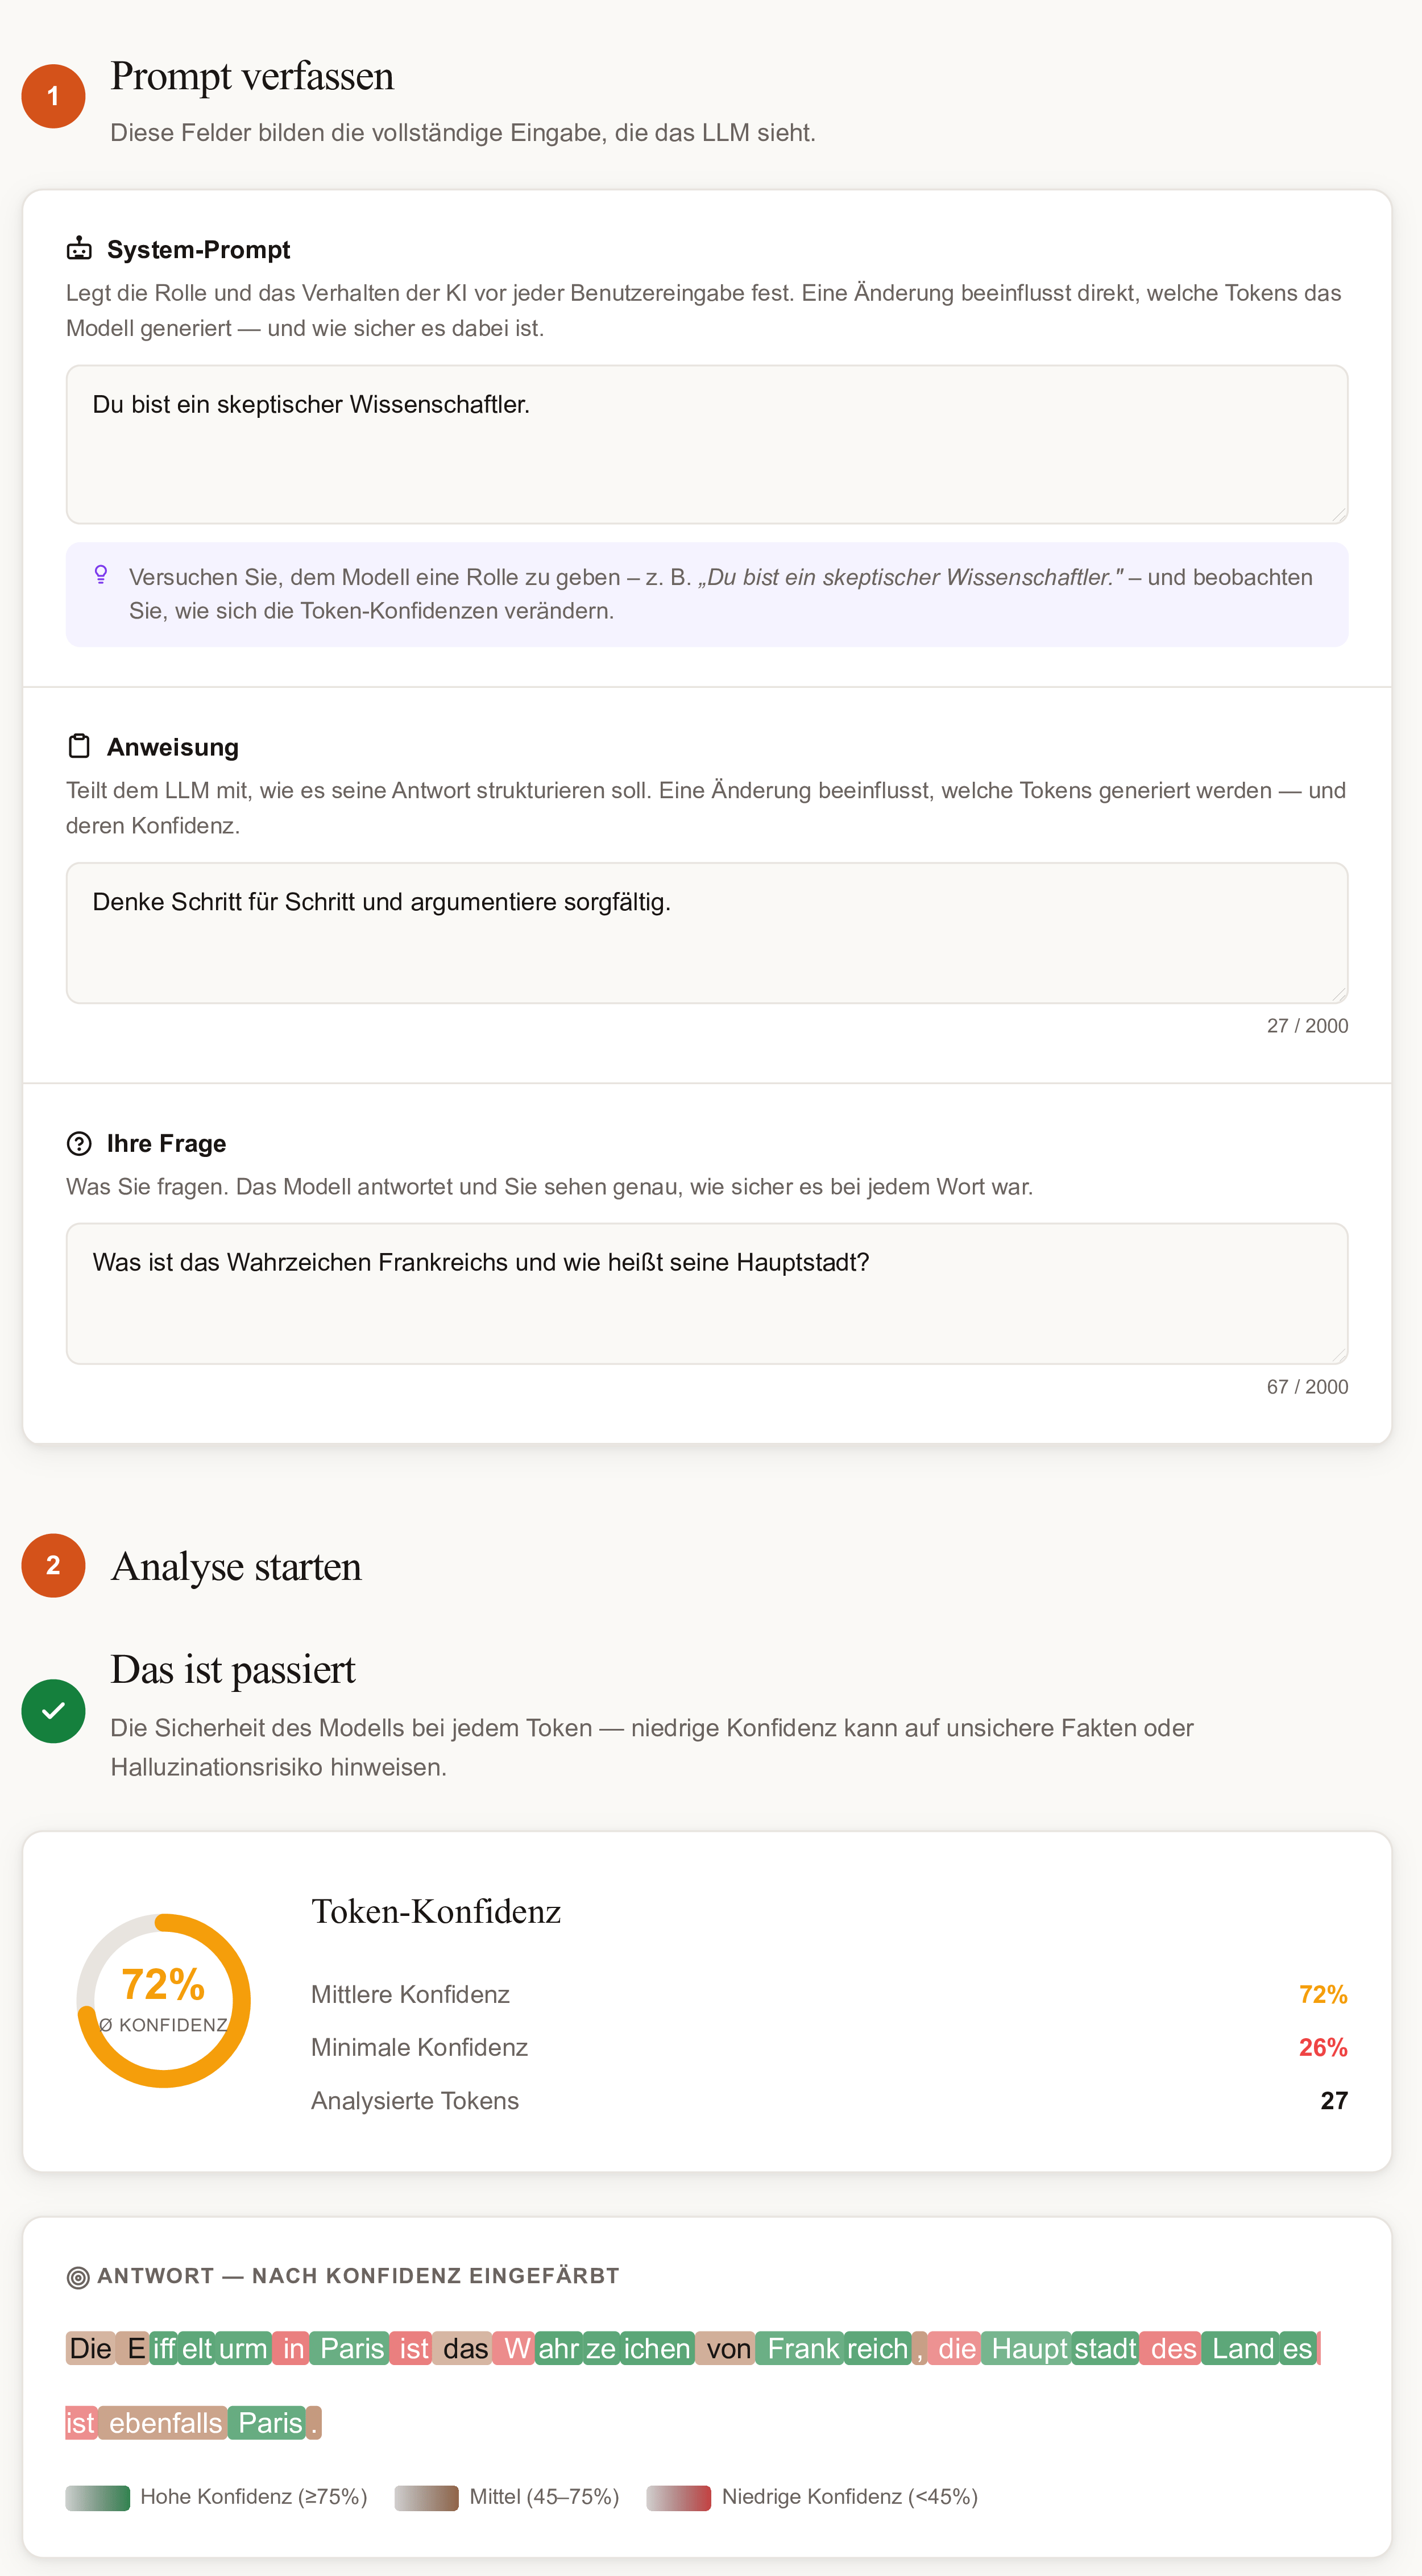
\includegraphics[width=0.7\linewidth]{img/conf_example.png}
    \caption{Confidence Sample}
    \label{fig:conf_sample}
\end{figure}
\FloatBarrier
\section{Empirical User Study}
\label{sec:empUserStudy}

The empirical component of this work consists of a structured online survey designed to measure how exposure to different XAI methods affects participants' trust in LLM-generated responses. The survey was administered via Tivian UniPark\cite{noauthor_online_nodate}, a professional survey platform that supports complex branching logic, randomization, and scaled response formats. Participants were recruited through the Bilendi panel service\cite{technology_bilendi_nodate}, which offers access to a broad pool of registered survey respondents across demographic groups, and which also provided feedback on the survey design prior to execution. This approach was chosen primarily for its cost-effectiveness and the speed with which a sufficient sample could be assembled.

The target sample size was constrained primarily by budget. In terms of composition, the study aimed for a balanced distribution across age groups and genders, with the requirement that all participants had prior experience using LLMs. The Bilendi panel allowed these filters to be applied at the recruitment stage.

\subsection{Survey Design}

Figure~\ref{fig:survey_flow} provides a complete overview of the survey flow. The survey is structured in three main phases: a background and screening phase, a core research phase in which trust is measured before and after exposure to XAI methods, and a closing reflection. Each phase is described in detail below.

\begin{figure}[p]
    \centering
    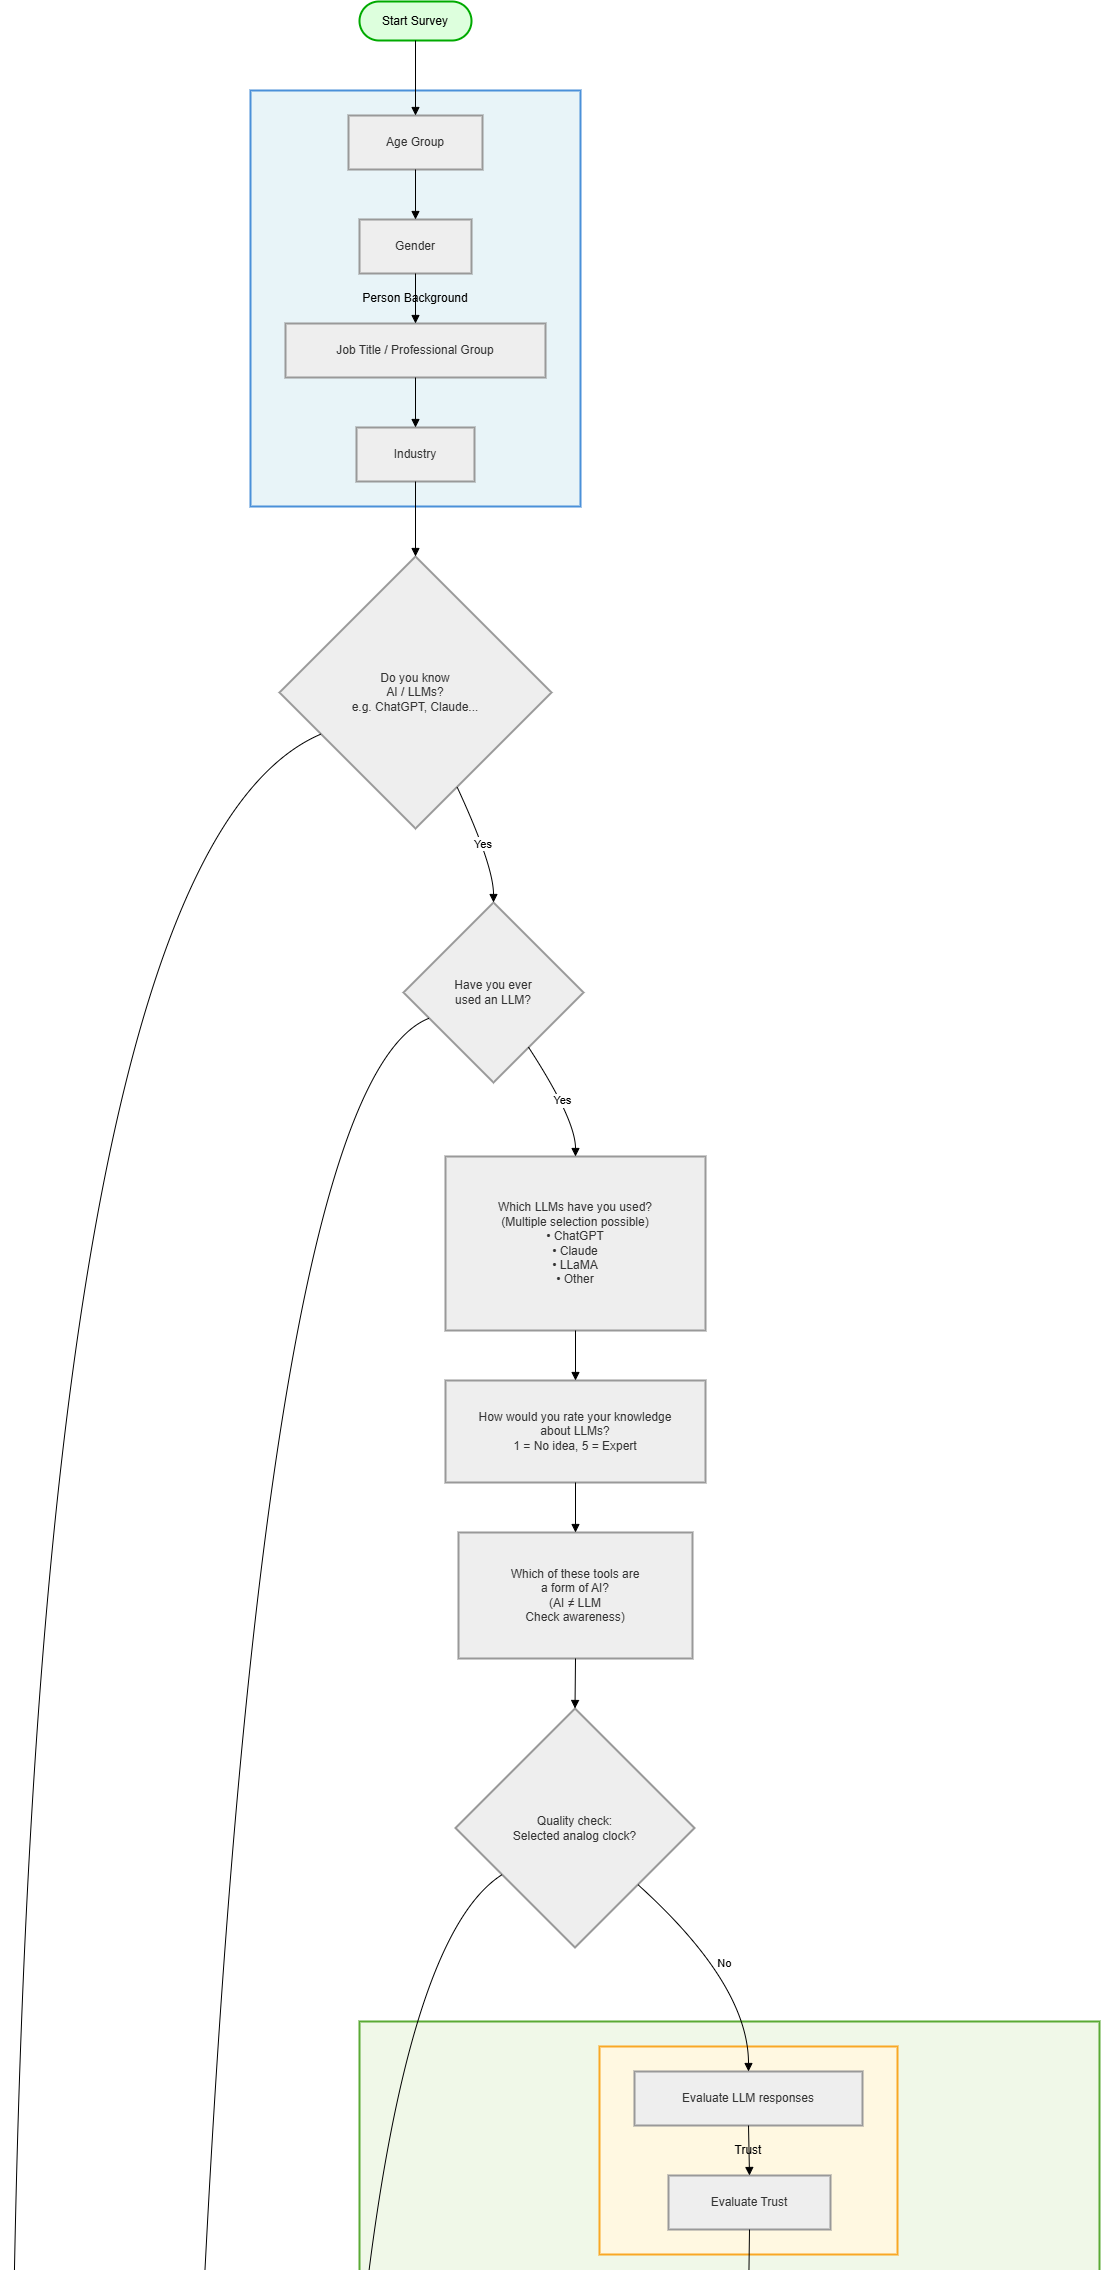
\includegraphics[width=0.7\linewidth]{img/survey_flow_p1.png}
\end{figure}
\begin{figure}[p]
    \centering
    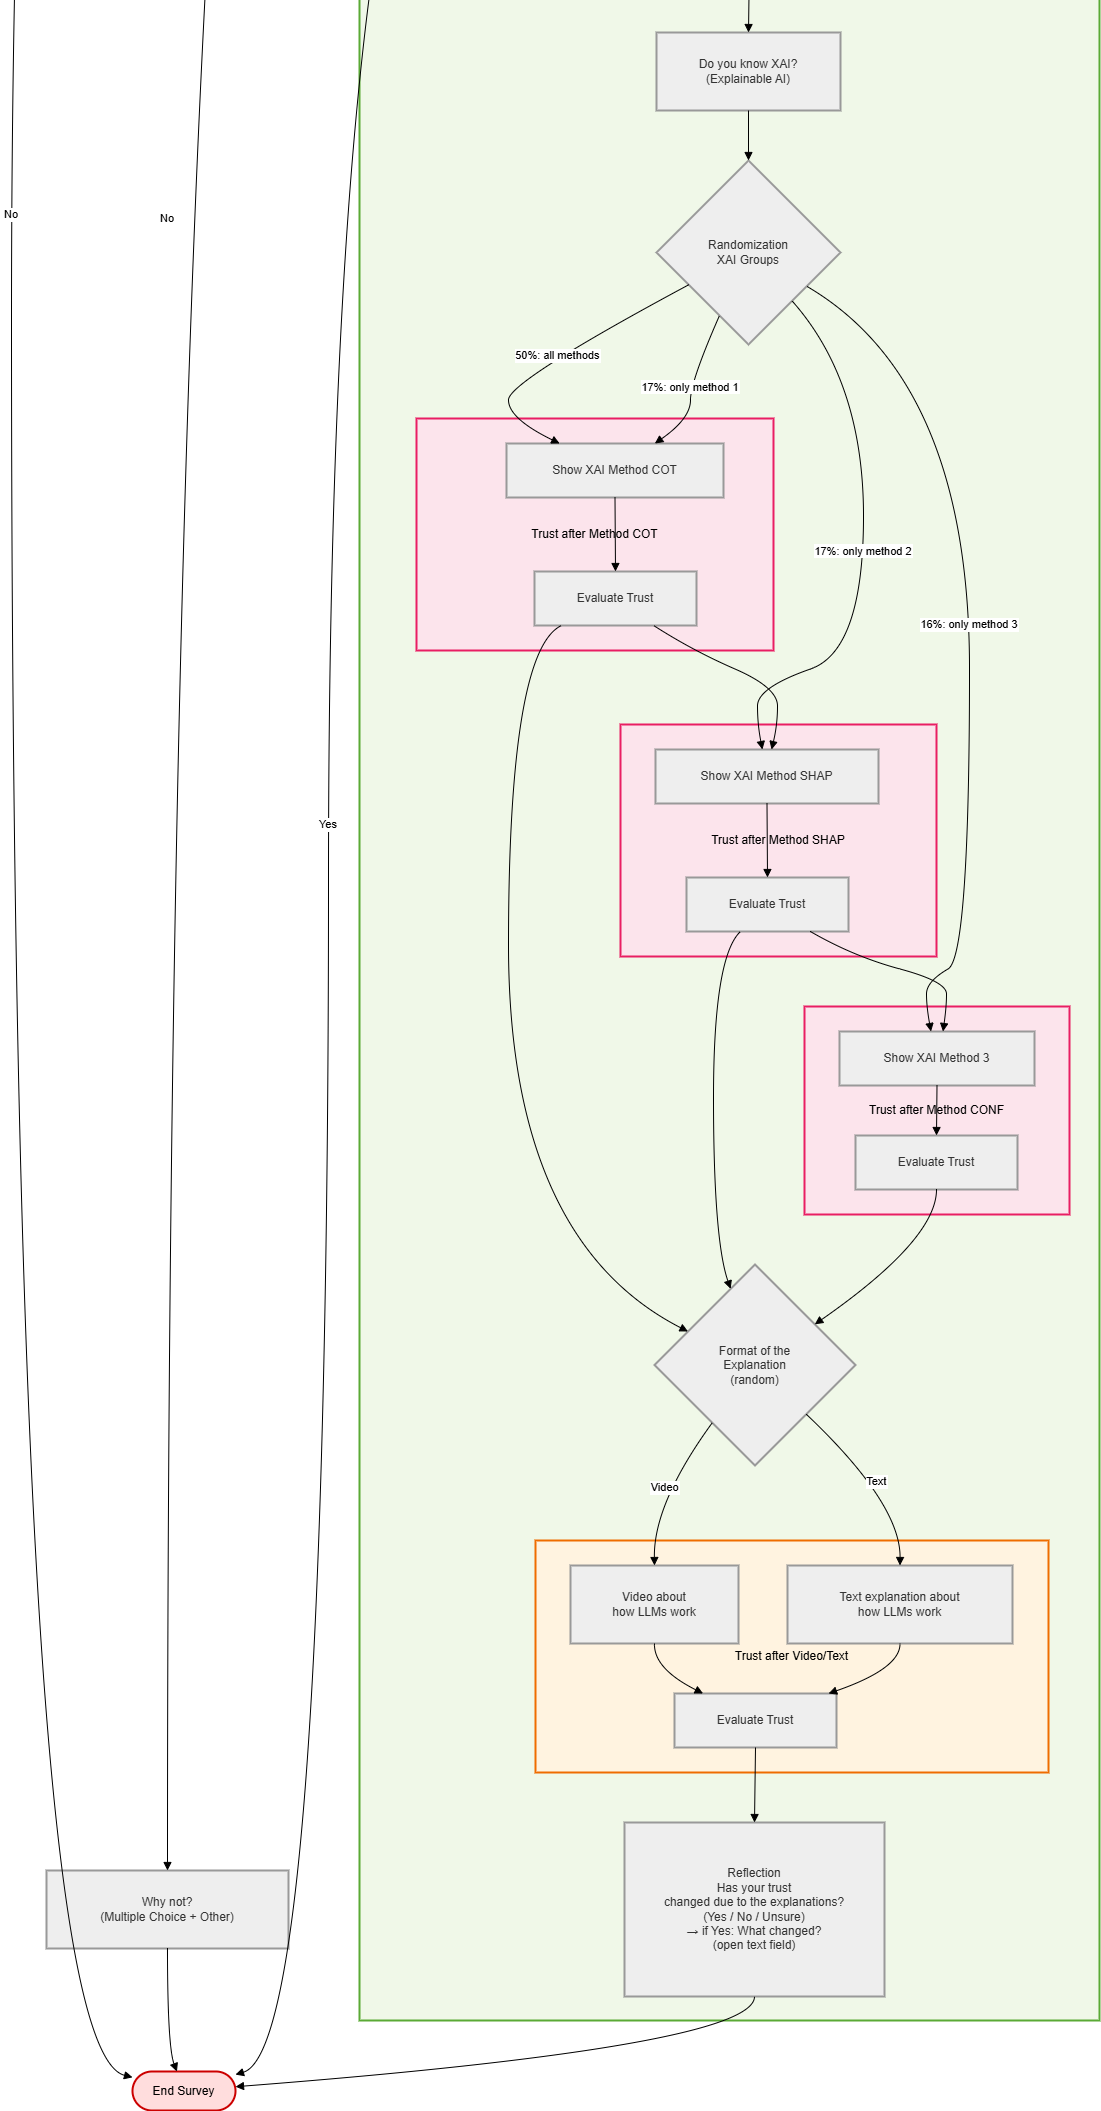
\includegraphics[width=0.7\linewidth]{img/survey_flow_p2.png}
    \caption{Survey Flow}
    \label{fig:survey_flow}
\end{figure}

The complete survey instrument, including all questions and branching logic, is reproduced in Appendix~\ref{appendix:survey}.
\subsubsection{Background and Screening}

The survey opens by collecting basic demographic information, including age group, gender, job title and occupational group, and industry. This is followed by two branching filter questions. Participants who indicate that they are not aware of AI or LLMs, with ChatGPT, Claude, and similar systems given as examples, are routed out of the survey, as are participants who have never used an LLM. Participants in the latter group are additionally asked an open-ended multiple-choice question about their reasons for non-use before being exited, providing supplementary data.

Participants who pass these filters proceed to report which LLM systems they have previously used, and to rate their self-assessed level of LLM knowledge on a five-point scale ranging from no knowledge to expert. A subsequent item asks participants to identify which of a list of tools constitute a form of artificial intelligence. This item serves a dual purpose: it probes awareness of the distinction between AI broadly and LLMs specifically, and it embeds a quality control check. Participants who select an analogue clock, an item that is clearly not a form of AI, are identified as inattentive and excluded from the analysis. This attention filter was implemented to improve data quality without relying on separate, easily identifiable attention-check items that experienced panel respondents may recognize and game.

\subsubsection{Use Case Categories and LLM Outputs}

Participants are next presented with a set of LLM-generated responses and asked to evaluate them. The responses were drawn from three thematic categories, selected to represent a range of contexts in which trust and accuracy carry meaningfully different stakes. The first category covers queries with potential legal implications, such as questions about whether certain activities are permitted, a domain where incorrect information could have direct personal consequences. The second category covers medical and health-related knowledge, where the reliability of information is similarly high-stakes. The third category covers general factual knowledge, which serves as a lower-stakes baseline. Importantly, the response set also includes factually incorrect LLM outputs, allowing the study to examine whether XAI methods help or hinder participants' ability to detect errors.

\subsubsection{Trust Measurement Instrument}
\label{sec:trust_instrument}

The construct of trust was operationalized based on a review of relevant literature on human-computer trust, as discussed in Section~\ref{sec:trust_theory}. Drawing on established theoretical distinctions, the instrument was designed to capture four different dimensions of trust: trust in the environment and the sociotechnical infrastructure, trust in the agent and any mediating agents, trust in potential interaction partners, and trust in authoritative sources \cite{castelfranchi_trust_2001}\cite{falcone_social_2001}\cite{jones_concept_2002}.

From these dimensions, a five-item scale was derived to assess trust responses to the system's outputs. Each item was rated on a five-point Likert scale ranging from \textit{stimme überhaupt nicht zu} (strongly disagree) to \textit{stimme voll zu} (strongly agree). The items were as follows:

\begin{itemize}
    \item \textit{Ich vertraue darauf, dass diese Antworten faktisch korrekt sind.} (I trust that these answers are factually accurate.)
    \item \textit{Ich halte die Informationen in diesen Antworten für zuverlässig.} (I consider the information in these answers to be reliable.)
    \item \textit{Diese Antworten wirken kompetent und sachkundig.} (These answers come across as competent and knowledgeable.)
    \item \textit{Ich glaube, dass das System versucht hat, korrekte Antworten zu geben.} (I believe the system has tried to provide accurate answers.)
    \item \textit{Ich würde mich bei diesen Antworten auf die enthaltenen Informationen verlassen.} (I would rely on the information contained in these answers.)
\end{itemize}

These items collectively capture multiple facets of trust, including perceived accuracy, reliability, competence, intentionality, and behavioral reliance. This repeated-measures design allows the effect of each XAI method on the full trust construct to be assessed across all five dimensions simultaneously.

\subsubsection{Randomization into XAI Groups}

After the baseline trust measurement, participants are informed about the concept of Explainable AI. They are then randomly assigned to one of four conditions. Approximately half of participants are shown all three XAI methods in sequence (CoT, SHAP with counterfactual, and confidence indication), while the remaining three groups are each shown only one of the three methods. This design allows both within-subject comparisons across methods for the full-exposure group and between-subject comparisons across the single-method groups, supporting more robust conclusions about the relative impact of each approach. Participants assigned to view all methods are additionally asked to rank them according to their perceived usefulness.

\subsubsection{LLM Explanation for Participants}

Following the XAI exposure and trust ratings, participants are randomly assigned to receive either a short video or a written text explanation of how large language models work, with both formats covering equivalent content in approximately three minutes. The aim is to convey a functional understanding of LLMs sufficient to contextualize the tasks they have completed, while avoiding overly technical language. Crucially, both formats emphasize that LLMs operate through statistical pattern matching rather than genuine understanding or intelligence, in order to correct potential anthropomorphization. Based on the mentioned criteria, this \href{https://www.youtube.com/watch?v=8Rumn1O-RkY}{\underline{video}} and this \href{https://axels-technikblog.de/was-ist-ein-llm-large-language-models-einfach-erklaert/}{\underline{textual explanation}} were chosen.
A final trust measurement is taken after this explanation, allowing any additional effect of the explanatory format, whether video or text, to be assessed.

\subsubsection{Reflection and Close}

The survey concludes with a brief reflection item that asks participants whether their trust in LLM outputs has changed as a result of the explanations they received, with response options of yes, no, and unsure. Participants who indicate that their trust has changed are invited to elaborate in a free-text field. This qualitative supplement enriches the quantitative trust data and may surface mechanisms of trust change that the scaled items do not fully capture.

\subsubsection{Data Quality Controls}

Beyond the attention filter embedded in the AI awareness item described above, a second quality control measure was applied: participants who completed the survey significantly faster than the median completion time, so-called ``speeders'', were excluded from the analysis. Anomalously short completion times are a reliable indicator that items were not read carefully. Both exclusion criteria were defined prior to data collection to avoid post-hoc rationalization of exclusions.

\section{Limitations}
\label{sec:limitations}

The primary limitation of this study concerns the generalizability of its findings. Although the Bilendi panel provides access to a large pool of respondents and allows filtering by demographic characteristics and prior LLM usage, the sample is ultimately composed of individuals who have registered to participate in online surveys for compensation. This introduces a self-selection bias: participants are not representative of the general population or of all LLM users, but rather of a specific subgroup willing to engage in panel research. Findings should therefore be interpreted with appropriate caution when generalizing beyond this population. Future work could address this limitation through more controlled recruitment strategies, including stratified sampling or in-person study designs.

\section{Prototype Implementation}
The resulting best xai method has been implemented like this

TODO.